\chapter{Introduction}

Hydrogen atom transfer (HAT) reactions involve chemical species with an odd
numbers of electrons, or free radicals. These fundamental chemical
transformations have been studied extensively for over a
century.\cite{Kochi1973,Parsons2000} All HAT reactions involve the transfer of
at least one hydrogen atom (\ch{H^.}), although there exist various mechanisms
by which this can occur. Free radicals and HAT reactions play an important role
in many chemical and biological processes.\cite{Halliwell2015} This chapter is
meant to serve as a brief summary of the importance and prevalence of HAT
reactions and the different factor which influence these reactions, in addition
to stating the research goals associated with this thesis.


\section{Physico-chemical determinants of formal hydrogen transfer reactions}

\subsection{Mechanistic details of hydrogen transfer reactions}

Given a simple HAT reaction, as shown in \ref{fig:hat}, there exists several
possible mechanisms by which this transformation can occur. The two most common
concerted mechanisms are hydrogen atom transfer (HAT)\cite{note1} ~and
proton-coupled electron transfer (PCET). At the basic level, HAT involves the
transfer of an electron and proton through the same set of acceptor/donor
orbitals, while PCET involves the transfer of an electron and proton through
different sets of orbitals. In practise, this distinction is poorly described
and this topic is still in active discussion in the
literature.\cite{Cukier1998,Mayer2002,Stubbe2003,Mayer2004,DiLabio2007,Huynh2007,
  Hammes-Schiffer2008,Mayer2010,Weinberg2012,Hammes-Schiffer2015,Munoz-Rugeles2017}
Primarily, the distinction between the two processes is unclear because the two
processes cannot be entirely separated physically.\cite{DiLabio2007}

\begin{scheme}[htb]
  \begin{center}
    \includegraphics[width=0.75\textwidth]{figures/FHT.eps}
  \caption{A generic formal hydrogen transfer reaction.}
  \label{fig:hat}
  \end{center}
\end{scheme}

The quintessential example when comparing HAT to PCET is the self-exchange
reactions of benzyl/toluene and phenoxyl/phenol shown in \ref{fig:self1}, as
described by \citet{Mayer2002}.

% \begin{align}
% \ch{ % C6H5CH2-H + C6H5CH2^. &-> C6H5CH2^. + C6H5CH2-H} \label{eq:self1} \\ 
% \ch{ % C6H5O-H + C6H5O^. &-> C6H5O^. +C6H5O-H} \label{eq:self2}
% \end{align}


\begin{scheme}[htb]
\begin{center} 
  \textbf{A. }\\
    \includegraphics[width=0.75\textwidth]{figures/PhCH3-PhCH2.eps}\\ 
  \textbf{B. }\\
    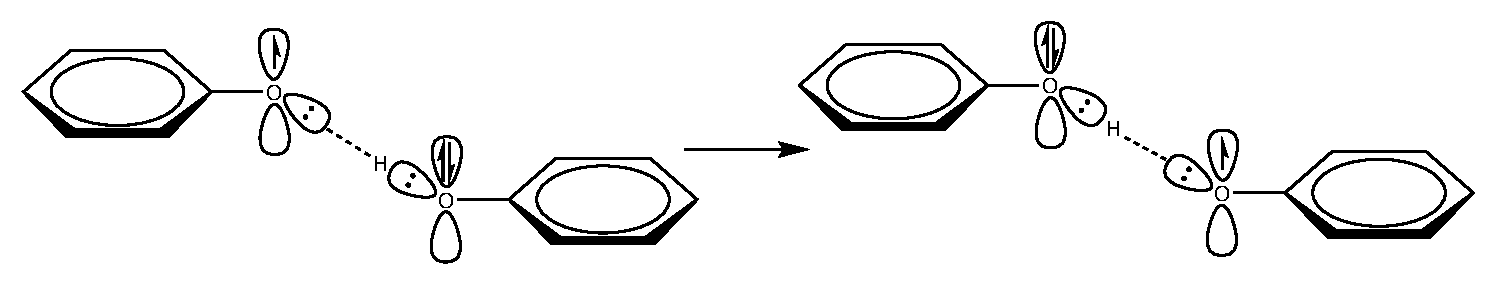
\includegraphics[width=0.95\textwidth]{figures/PhOH-PhO.eps}\\
    \caption{Self-exchange reactions of the \textbf{A.} benzyl/toluene couple
      through HAT \textbf{B.} phenoxyl/phenol couple through PCET.}
  \label{fig:self1}
\end{center}
\end{scheme}

In this work, the transition state structures, obtained through
density-functional theory (DFT) calculations were reported. The proposed
structures have $C_{2h}$ and $C_2$ symmetry for \ref{fig:self1} A and B,
respectively, oriented so that the aromatic rings are trans relative to one
another. In this geometry, the benzyl/toluene pair undergoes direct HAT, with
the $2p-\pi$ orbital of the benzylic carbon radical oriented at the benzylic
hydrogen on toluene and little delocalisation of the radical into the
$\pi$-system. Additionally, the singly occupied molecular orbital (SOMO) is of
$\sigma$ symmetry. This reaction has a calculated enthalpic barrier
($\Delta H^{\ddagger}$) of 17.7 kcal/mol. For the phenoxyl/phenol pair, a fairly
strongly hydrogen bonded pre-reaction complex is first formed (-8.1 kcal/mol,
relative to reactants). The TS structure is such that the phenoxyl radical in a
$2p$ orbital is allowed to overlap with $2p$ lone pair of phenol moiety and the
aromatic $\pi$ systems, so that the SOMO is of $\pi$ symmetry and highly
delocalised. This indicates a PCET mechanism, and the reaction has a barrier
height $\Delta H^{\ddagger}$ = 5.0 kcal/mol relative to the hydrogen bonded
complex, so that the barrier is 3.1 kcal/mol below the separated reactants.

\jnote{Another example is iminoxyl / oxylimine self-exchange \cite{DiLabio2005},
include if another example would be useful}

% \begin{align}
 % \ch{ R2C=N^.-O + H-O-N=CR2 -> R2C=N-O-H + O-N^.=CR2} \label{eq:self3}
% \end{align}

The work by \citet{Mayer2002} suggests that hydrogen bonding is a necessary, but
not sufficient condition for PCET to occur. This then implies that PCET not
possible between molecules which do no possess hydrogen bonding moeities, such
as carbon atoms. Work by other authors has shown this to be
untrue.\cite{Hatcher2007,DiLabio2007} In particular, \citet{DiLabio2007}
demonstrated that this neglected the important contributions of $\pi-\pi$
interactions and lone pair-$\pi$ interactions. This was achieved by showing
there exits a TS structure for the benzyl/toluene couple which is 3.7 kcal/mol
lower in energy than previously reported. This structure has $C_2$ symmetry
with the aromatic rings oriented $34^\circ$ relative to one another, allowing
for optimal $\pi$-stacking and that there the $\pi$-$\pi$ overlap opens up an
electronic channel for PCET to occur. This was confirmed by
\citet{Munoz-Rugeles2017}, who, using an approach which utilises natural
population analysis along the intrinsic reaction coordinate, showed that both the
benzyl/toluene couple and phenoxyl/phenol couple favour a $\pi$-stacked TS
structure and undergo transfer through a PCET mechanism.\jnote{Long sentence}
Interestingly, they also showed that reaction barriers heights for the PCET
mechanism are systematically lower than those for formal HAT.

As there is not obvious way to explore the differences in mechanism
experimentally, computational examination of formal HAT reactions enables
analysis of the mechanism of these reactions. Using a variety of tools, a
general distinction between a HAT mechanism and PCET mechanism can be achieved,
however, as stated previously, these mechanisms are not mutually
exclusive. Regardless, important insight can be gained from understanding the
electronic behaviour of these reactions.


\subsection{The influence of bond strengths on HAT reactions}

It has long been the interest of chemists to understand chemical reactions from
both a thermodynamic and kinetic stand-point. The measurement and comparison of
bond strengths, that is bond dissociation enthalpies (BDEs), is central to the
understanding of reactivity with respect to thermodynamics. There exists a
tremendous amount of literature in which BDEs are linked to chemical reactivity,
especially for HAT
reactions.\cite{Kochi1973,Tedder1982,Wijtmans2003,Pratt2004,Mayer2004}

Often, BDEs are used in linear free energy relationships (LFERs) to relate
chemical reactivity to bond strength. One such example\cite{Pratt2004} is the
application of BDEs to the Hammett equation\cite{Anslyn2006}, which can be used
to study substituent effects from thermodynamic (Equation
\ref{eq:hammettthermo}) or kinetic analysis (Equation \ref{eq:hammettkin}).

\begin{align}
 \log\frac{K_X}{K_H} &= \rho \sigma_X \label{eq:hammettthermo} \\
 \log\frac{k_X}{k_H} &= \rho \sigma_X \label{eq:hammettkin}
\end{align}

\noindent In the above equations, $K$ is an equilibrium constant and $k$ is a
rate constants for either a reference reaction with a hydrogen substituent $H$
or a given substituent $X$. The substituent parameters $\sigma_X$, have been
measured for various different reference reactions, although the original
parameters were measured for the acidity of benzoic acid.\cite{Hammett1937}
~Plots of $\log(K_X/K_H)$ or $\log(k_X/k_H)$ against $\sigma_x$ have be used to
determine $\rho$, the sensitivity constant, which originally was used to determine
whether a reaction was more sensitive ($\rho > 1$), less sensitive ($\rho < 1$),
or equally sensitive to substituents than benzoic acid, with negative charge
being produced. If $\rho$ is negative then positive charge is said to be formed as a
result of substituents.

In the context of BDEs, \citet{Pratt2004} examined a series of substituents (Y)
on toluenes, anilines, and phenols (4-\ch{YC6H4-ZX}), and showed that the Z-X
BDEs can be correlated to the electrophilic substituent constants,
$\sigma_p^+$(Y). This was surprising since it demonstrated that homolytic
properties correlated with properties derived from the heterolytic $S_N1$
solvolyses of para-substituted cumyl chlorides.\cite{Brown1958} Specifically,
this showed that since $\sigma_p^+$(Y) describes the relative ability of Y to
stabilise a positive charge, the ability to stabilise strong electron
withdrawing (EW) moieties can be well described in general by these
parameters. This means that BDEs for toluenes and anilines are well correlated
to $\sigma_p^+$(Y), since \ch{O^.} and \ch{NH^.} can be described like positive
charges (strong EW groups). Toluenes, which have resulting radicals (\ch{CH2^.})
which are neither electron withdrawing or donating, are poorly correlated with
$\sigma_p^+$(Y).

Another interesting LFER, which is utilised in Chapter \ref{ch:bdes}, is the
Bell-Evans-Polanyi (BEP) Principle,\cite{Bell1936,Evans1938} which states that
the difference in activation energy ($E_a$) for two related reactions (within
the same family), is proportional to the differences in reaction enthalpy
($\Delta H$): Equation \ref{eq:bep}.

\begin{align}
  E_a = E_0 + \alpha \Delta H
  \label{eq:bep}
\end{align}  

\noindent This relationship has been more generally used to compare larger
families of reactions, such that he remaining terms are $E_0$, the activation
energy of a reference reaction, and $\alpha$ is a constant which characterised
the position of the TS along the reaction coordinate. This can be rationalised
by considering a series of reactions with similar energy profiles: if the
reaction becomes more exothermic, the barrier height will decrease (the opposite
is also true for endothermic reactions), as illustrated in \ref{fig:bep}. 

\begin{figure}[htb]
  \centering
  \includegraphics[width=0.7\textwidth]{figures/bep}
  \caption{Energy profiles for a series of related exothermic reactions
    illustrating the Bell-Evans-Polanyi Principle.}
  \label{fig:bep}
\end{figure}

If the BEP relationship holds for a series of related HAT reactions, then BDEs
should correlate with the activation energy. More commonly, plots of BDEs
against the logarithm of rate constant are used. An interesting example of this
is the work of \citet{Pratt2003}, in which the free radical oxidation of
unsaturated lipids is examined. They achieve this through the correlation of
theoretically determined C-H and \ch{C-OO^.} bond strengths with experimentally
measured HAT rate constants and \ch{O2} addition rate constants,
respectively. BEP plots (BDE vs. $\log k$) for a large range of polyunsaturated
fatty acid models show good correlation for both the C-H bonds and \ch{C-OO^.}
bonds examined. This demonstrated that BDEs have a direct impact on the reaction
barrier height, giving validation to the BEP Principle.

Although chemists often consider the importance of BDE in thermodynamic
analysis, bond strengths are an important consideration in kinetic analysis as
well. As such, the altering of bond strengths can be an important factor in
related HAT reactions.

\subsection{Stereo-Electronic contributions to HAT reactions}

The effects of sterics and electronics have been shown to play an important role
in HAT reactions. Generally, these effects are described as two seperate
phenomena: Polar effects and steric effects.

The species involved in HAT reactions are often neutral radicals, thus the
influence of charge transfer in the TS complex can have important
implications. Consider the TS of a generic HAT reaction in \ref{fig:hatts},
there are four obvious resonance forms. For a series of related reactions, $E_a$
would be expected to decrease as the contribution of dipolar ion resonance forms
increases.\cite{Roberts1999} Oxygen centred radicals, as is the focus of our
work, are electrophilic in nature, thus the importance of the third resonance
structure becomes important. This is important, as HAT is be favoured at C-H
bonds which are electron rich, or nucleophilic.\cite{Salamone2015Rev}

\begin{scheme}[htb]
  {\huge\ch{[X-H-Y]}$^\ddagger$} \\
  \vspace{0.5cm}
  {\large
  \ch{[X^.H-Y]}$^\ddagger$ \ch{<-> [X-H Y^.]}$^\ddagger$ \ch{<->
    [X:^-H^.Y^+]}$^\ddagger$ \ch{<-> [X^+H^.Y:^-]}$^\ddagger$} 
  \caption{A generic HAT transition state structures and possible resonance forms.}
  \label{fig:hatts}
\end{scheme}  

An  example   of  this   effect  is   from  the  work   of  our   colleagues  in
Rome,\cite{Bietti2011,Salamone2012} in  which rate constants  ($k_H$, normalised
for the  number of abstractable  hydrogens) for  cyclohexane and acetone  to the
cumyloxyl radical (\cumo) were measured and compared to theoretically determined
C-H BDEs. Cyclohexane has a C-H BDE  = 99.5 kcal/mol and $k_H$ = $9.2\times10^4$
\Ms, while  acetone has C-H BDE  of 96.0 kcal/mol  and $k_H$ = $  < 2\times10^3$
\Ms. As a result of polar effects, although cyclohexane has a much stronger bond
strength,  it is  at least  an  order of  magnitude  more reactive  in HAT  than
acetone.  Note  that it is these  polar effects which also  enable polar aprotic
solvents to be used in typical  physical organic experiments which measured rate
HAT rate  constants (laser  flash photolysis  (LFP), for  example), as  the rate
constants are typically much smaller than  those of the substrate which is being
characterised.

The effects of steric bulk also play an important role in HAT, and have been
studied extensively by our colleagues in Rome, as well as by
others.\cite{Finn2004,Salamone2011,Pischel2001,Griller1981,Bietti2011,Salamone2012,Malatesta1982,Salamone2014}
Although a C-H bond may be weaker than others on a given substrate, if it is not
accessible due to steric constraints, abstraction will not occur at this
site. Otherwise, additional steric bulk can lead to significant reductions in
reactivity. For example, reactions of tertiary acetamides with
\cumo,\cite{Salamone2014} where abstraction occurs mainly from C-H bonds
$\alpha$ to the nitrogen atom, a two fold decrease in normalised rate constant
is observed in going from N,N-dimethylacetamide to N,N-diisobutylacetamide
($k_H$ = $2.0 \times 10^5$ and $7.8 \times 10^4$ \Ms, respectively).

It is worth noting that there is some dispute whether bond strengths are the
most important factor in HAT reactions. Specifically, the work of Zavitsas\cite{Zavitsas1995,Zavitsas2012}
outlines that the most important feature in determining $E_a$ for a HAT reaction
is the parallel alignment of spins in the TS complex, or ``triplet repulsion'',
shown in \ref{fig:tripletrep}.

\begin{scheme}[htb]
  \centering
  {\huge [\ch{X ^ \bond{single} H v \bond{single} Y ^}]$^\ddagger$} OR~
  {\huge [\ch{X v \bond{single} H ^ \bond{single} Y v}]$^\ddagger$}
  \caption{Prototypical hydrogen atom transfer transition state demonstrating
    triplet repulsion.}
  \label{fig:tripletrep}
\end{scheme}

\jnote{I realise that this could be just another way to describe/extension of
  the polar effects described above, so I opted to not write more than
  this. Should they be combined or should I exclude this all together?}

\subsection{The effects of medium on HAT reactions}

Although computational chemistry allows the study of HAT reactions on the single
molecule level, experimentally this is not feasible and the effects of solvent
and other media are important to factor into the understand of these
reactions. The most characterised kinetic solvent effects (KSEs) have been
characterised for phenols. Early studies of reactions involving the oxidation of
styrene in the presence of phenols and peroxyl radicals,\cite{Howard1964} as
described by Equations \ref{eq:ox1} and \ref{eq:ox2}, an increase in the ratio
of rate constants was observed with increasing solvent polarity.

\begin{align}
  \ch{ROO^. + RH &-> ROOH + R^.} \label{eq:ox1} \\
  \ch{ROO^. + ArOH &-> ROOH +  ArO^.} \label{eq:ox2}
\end{align}

\noindent This change was attributed to the reduction in the rate constant of
Equation \ref{eq:ox2} as a result of hydrogen bond (HB) formation of phenol with
HB-accepting (HBA) solvents. This was further validated in LFP
experiments\cite{Das1981} for the reaction of phenols with $tert$-butoxyl
radicals. The rate constants for phenol were found to be $3.3 \times 10^8$ \Ms
in benzene and $4.7 \times 10^6$ \Ms in pyridine, demonstrating that KSEs are
significant, especially when HB formation is involved.

The systematic investigation of KSEs lead to the development of the empirical
Snelgrove-Ingold equation\cite{Snelgrove2001,Litwinienko2007} (Equation
\ref{eq:kse}), which when given the rate constant for reference solvent ($k^0_H$),
quantitatively describes KSEs for HAT from phenols, hydroperoxides, anilines,
and hydrocarbons according to the ability of the substrate to donate a hydrogen
bond and the ability of the solvent to accept hydrogen bonds.

\begin{equation}
  \log(k_H^S) = \log(k_H^0) - 8.3\alpha_2^H_{subst}\beta_2^H
  \label{eq:kse}
\end{equation}

\noindent In this equation, the ability of the substrate to hydrogen bond donate
(HBD) is measured by $\alpha_2^H_{subst}$, the so called Abraham HBD
parameters,\cite{Abraham1989} and the HBA capability of the solvent in measured
by the Abraham HBA parameters $\beta_2^H$.\cite{Abraham1990} Plots of
log($k$,\Ms) against $\beta_2^H$ are used as a LFER to quantify KSEs and give
good correlations for the HAT reactions described above, and other reactions
such as the radical/radical reaction \ref{eq:hoohoo}:\cite{Foti2005}

\begin{equation}
  \ch{HOO^. + HOO^. -> HOOH + O2}
  \label{eq:hoohoo}
\end{equation}

The success of this equation can be ascribed to the description of how KSEs act
on the kinetics of the reaction, described by \ref{fig:kse}.

\begin{scheme}[htb]
  \includegraphics[width=0.75\textwidth]{figures/kse.eps}
  \caption[The kinetic solvent effect on HAT reaction]{The kinetic solvent
    effect on HAT reaction. Figure adapted from Reference
    \citenum{Litwinienko2007}.}
  \label{fig:kse}
\end{scheme}

\noindent In this description, there is an equilibrium between the free and
solvent bound substrate, where HB-ing disallows the HAT reaction. This
description requires three assumptions: (i) Each X-H substrate molecule can HB
with one molecule of HBA solvent, S. (ii) The equilibrium constant for HB
formation ($K_{XH/S}^S$) is independent of the surrounding mediums
properties. (iii) HAT cannot occur from the bound substrate, for steric reasons,
and only free X-H can react with a radical, \ch{Y^.}. The HAT reaction can
proceed when X-H is free, and possesses a characteristic rate constant
($k_{XH/\ch{Y^.}}^0$) equal to the measured rate constant in non-HBA
solvent. According to this, the experimental rate constant in a HBA solvent can
be determined by

\begin{equation}
  k_{XH/\ch{Y^.}}^S = k_{XH/\ch{Y^.}}^0/(1+K_{XH/S}^0)
  \label{eq:ksek}
\end{equation}

Further evidence for the success of the Snelgrove-Ingold equation can be seen in
successful application to KSE studies of various phenols and $\alpha$-tocopherol
with tert-alkoxyl,\cite{Valgimigli1995,Avila1995,MacFaul1996,Snelgrove2001}
peroxyl,\cite{Jha2008} and diphenyl-1-picrylhydrazyl (\ch{DPPH^.})
radicals,\cite{Valgimigli1995,Valgimigli1999} and the reaction of tert-butyl
hydroperoxide with \cumo,\cite{Snelgrove2001,Avila1995} amongst many
others.\cite{Litwinienko2007,Bietti2012} It is worth noting that this
description neglects the effects of HB-ing to the abstracting radical species in
the HAT reaction. There does not appear to be any clear quantification of this
effect, however work by \citet{Bietti2012}, which studies the HAT between \cumo
and phenol, showed that the Snelgrove-Ingold equation overestimated the rate
constants measured in trifluoroethanol (TFE), acetonitrile (MeCN) mixed with
\ch{H2O} (2:1), and methanol. This implies that solvent HB-ing to radicals
can play a non-negligible role.

For KSEs on HAT from C-H bonds to oxygen centred radicals, as is the focus of
this thesis, effects are generally smaller than for phenolic
substrates. \citet{Salamone2014Syn} have described these interactions as an
interplay of solvent/substrate and solvent/radical hydrogen bonding. For
hydrocarbon HAT with \cumo, $k_H$ was found to be nearly solvent independent in
aprotic solvents.\cite{Bietti2010,Bietti2011,Avila1993} (1.1-1.2 $\times 10^6$
\Ms for cyclohexane) With strong HBD solvents, however, an increase in $k_H$ was
observed. (Cyclohexane = $4.4 \times 10^6$ \Ms in TFE) This effect can be traced
back to the polar effects described above, where the TS for HAT experiences
charge transfer such that the radical oxygen has partial negative charge, giving
the oxygen greater $sp^2$ character. Due to this, hydrogen bonding increases in
strength along the reaction coordinate and the TS is stabilised, relative to the
reactants, thus $k_H$ increases. This effect is also observed in the primary
decay pathway of \cumo, by means of $\beta$-scission as shown in
\ref{fig:cumobeta}.\cite{Avila1993}

\begin{scheme}
  \includegraphics[width=0.75\textwidth]{figures/cumobeta}
  \caption{The $\beta$-scission of \cumo}
  \label{fig:cumobeta}
\end{scheme}

In additional work by our Roman colleagues, it was demonstrated that C-H bond
HAT substrates which have HBA accepting capabilities, $k_H$ was observed to
decrease with solvent HBD ability. Evidence for this is summarized in \ref{tab:kse}.


\begin{table}[htb]
{\footnotesize
%  \begin{adjustwidth}{-7mm}{}
\centering
  \begin{tabular}{l r r r}
    Solvent & $N,N$-dimethylformamide$^a$ & Tetrahydrofuran$^b$ & Triethylamine$^c$ \\
    \hline
    \hline
    isooctane & (7.7 $\pm$ 0.1) $\times 10^6$ & (1.21 $\pm$ 0.02) $\times 10^7$ & \rule{0pt}{3ex} (2.9 $\pm$ 0.1) $\times 10^8$  \\
    benzene & (3.1 $\pm$ 0.1) $\times 10^6$ & (7.2 $\pm$ 0.7) $\times 10^6$ & (2.8 $\pm$ 0.1) $\times 10^8$ \\
    MeCN & (1.24 $\pm$ 0.02) $\times 10^6$ & (5.8 $\pm$ 0.2) $\times 10^6$ & (2.0 $\pm$ 0.1) $\times 10^8$ \\
    $t$-BuOH & (1.38 $\pm$ 0.03) $\times 10^6$ & (5.8 $\pm$ 0.2) $\times 10^6$ & (1.61 $\pm$ 0.03) $\times 10^8$ \\
    MeOH & (9.8 $\pm$ 0.2) $\times 10^5$ & (4.9 $\pm$ 0.2) $\times 10^6$ & (3.8 $\pm$ 0.1) $\times 10^6$ \\
    TFE & $<$ 1 $\times 10^4$ & (2.7 $\pm$ 0.1) $\times 10^6$ & \\
  \end{tabular}
  \caption[Summary of second-order rate constants for HAT from C-H bonds for
  hydrogen bond accepting substrates from the cumyloxyl radical.]{Second-order
    rate constants ($k_H$, \Ms) for HAT from C-H bonds of hydrogen bond
    accepting substrates to the cumyloxyl radical measured in difference
    solvents at 25 $^{\circ}$C. $^a$Reference
    \citenum{Salamone2015}. $^b$Reference \citenum{Salamone2014Syn} and
    \citenum{Bietti2011}. $^c$Reference \citenum{Bietti2010}.}
  \label{tab:kse}
}
%  \end{adjustwidth}
\end{table}

\noindent In C-H bonds, especially those $\alpha$ to heteroatoms,
hyperconjugative overlap between the $\alpha$-C-H $\sigma^*$ orbital and the
neighbouring lone-pair is important. (See section on hyperconjugation in
POC:theory\jnote{include cross reference when available} for discussion
regarding hyperconjugation.) The KSE of C-H abstraction in HBD solvents has been
explained in terms of hyperconjugation: HB-ing decreases the degree of
hyperconjugative overlap, leading to an increase in the strength of the C-H
bond, thus destabilising the TS complex and incipient carbon radical and
corresponding to a decrease in $k_H$.\cite{Salamone2014Syn,Salamone2015Rev}

The experimental investigation of other Lewis acids on HBD substrates that react
through HAT with C-H bonds has been underway by the Bietti group in Rome. The
effects of non-redox active metal cations on HAT from C-H bonds of
cyclohexadiene(CHD), tetrahydrofuran (THF), and tertiary alkylamines to \cumo
were examined.\cite{Salamone2013} This work is summarized in
\ref{tab:expcations}. Additional experiments examining the same reactions of
$N,N$-dimethylacetamide (DMA) and $N,N$-dimethylformamide
(DMF)\cite{Salamone2015}, as well as for various other
acetylamides\cite{Salamone2016} have been performed, and provides the
experimental background for this thesis.

\begin{table}[htb]
  \centering
  \begin{tabular}{c l r}
 Substrate & Conditions & $k_H$(\Ms) \\
 \hline
 \hline
CHD & \rule{0pt}{3ex}            & (6.65 $\pm$ 0.02) $\times 10^7$ \\
        & \ch{LiClO4} 1.0 M       & (7.49 $\pm$ 0.04) $\times 10^7$ \\
        & \ch{Mg(ClO4)2} 1.0 M & (7.0 $\pm$ 0.1) $\times 10^7$ \\
\hline
THF  &                                    & (5.7 $\pm$ 0.1) $\times 10^6$ \\
        & \ch{LiClO4} 1.0 M       & (2.87 $\pm$ 0.04) $\times 10^6$ \\
        & LiOTf 1.0 M                & (2.8 $\pm$ 0.2) $\times 10^6$ \\
        & \ch{Mg(ClO4)2} 1.0 M & (1.8$\pm$ 0.1) $\times 10^6$ \\
\hline
TEA  &                      & (2.0 $\pm$ 0.1) $\times 10^8$ \\
        & \ch{LiClO4} 1.0 M           & (9.37 $\pm$ 0.01) $\times 10^7$ \\
        & \ch{Mg(ClO4)2} 0.005 M & $<$ 1 $\times 10^{6*}$ \\
\hline
PMP  &                                       & (1.70 $\pm$ 0.02) $\times 10^8$ \\
        & \ch{LiClO4} 1.0 M           & (9.0 $\pm$ 0.3) $\times 10^ 7$ \\
        & \ch{Mg(ClO4)2} 0.005 M & $<$ 1$\times 10^{6*}$
  \end{tabular}
  \caption[Summary of experimental rate constants of HAT with \cumo for
  cyclohexadiene (CHD), tetrahyrofuran (THF), triethylamine (TEA), and
  1,2,2,6,6-pentamethylpiperidine (PMP), including the effect of non-redox
  active metal cations.]{Summary of experimental rate constants of HAT with
    \cumo for cyclohexadiene (CHD), tetrahyrofuran (THF), triethylamine (TEA),
    and 1,2,2,6,6-pentamethylpiperidine (PMP), including the effect of non-redox
    active metal cations. Rate constants were determined by LFP in 25
    $^{\circ}$C MeCN. $^*$Rate constants are approximate as the effects of even
    small additions of metal cations cause to rate decreases below the range of
    LFP.}
  \label{tab:expcations}
\end{table}

In general, metal cation interactions lead to deactivation of C-H bonds and
experimental rate constants decrease as a result. This has been explained on the
same basis as for KSEs, where Lewis acid binding causes a decrease in
$\alpha$-C-H bond $\sigma^*$ population, thus increasing the effective C-H bond
strength and decreaing $k_H$. For cyclohexadiene, a marginal increase in $k_H$
was observed with additons of 1.0 M \ch{LiClO4} and \ch{Mg(ClO4)2},
demonstrating that metal cations have a limited ability to influence HAT
reactions of \cumo with alkene based substrates. For THF, $k_H$ is 2.0 and 3.2
times lower relative with the additon of 1.0 M \ch{LiClO4} and \ch{Mg(ClO4)2},
respectively. \ch{LiClO4} has a roughly 2-fold descreasing effect on $k_H$ for
alkylamines, whereas \ch{Mg(ClO4)2} has a significantly greater effect,
decreasing $k_H$ by more than two orders of magnitude. As a whole, these results
suggest that metal ions interact more strongly with substrates that \cumo, thus
a Lewis acid/base effect, as seen from hydrogen bonding is observed. The Lewis
acidity of the metal appears to have an important role, since \ch{Mg(ClO4)2} $>$
\ch{LiClO4} in regards to Lewis acidity and effect on $k_H$. The Lewis basicity
of the substrate is also clearly important, as a large increase in moving from
THF to alkylamines. Computational studies have validated these results,
demonstrating that \ch{Mg(ClO4)2} leads to a 5.1 kcal/mol decrease in the
$\alpha$-C-H BDE in triethylamine and that $k_H$ decreases by $>4$ orders of
magnitude.\cite{Nova2014}

Simple amides such as DMF and DMA are often used as simple peptide
models.\cite{Salamone2015a} As such the deactivation of C-H bonds in amides, as
indicated by the observed decreases in $k_H$, leads to the central hypothesis of
this thesis: \emph{non-redox active metals cations can serve as chemoprotective
  agents for biomolecules}. Experimental evidence for this is demonstrated in
\ref{fig:expdmadmf}. For \ch{LiClO4} added to DMF and DMA, total inhibition of
HAT occurs up to 2 and 1 molar equivalents, respectivly. Inhibition of HAT
occurs for 2 and 4 molar equivalents, respectively, followed total
non-inhibition. A much weaker effect is observed with \ch{NaClO4}, while a
similar strong deactivating effect is observed for \ch{Ca(ClO4)2}. The addition
of \ch{Mg(ClO4)2} gives weak deactivation for the first two molar equivalents of
both DMF and DMA, with strong activation for an additonal two equivalents. This
unusual behaviour is as of yet, unexplained.

\jnote{Include these figure as well? It seems like this data should maybe be
  collected and placed into the appendix (I'm unsure of how else to include this
  data given the different ranged of effects)}

\begin{figure}[htb]
  \centering
  \includegraphics[width=0.9\textwidth]{figures/exptdmadmf}
  \caption[Plots of observed rate constants against concentration of substrate for HAT
  reactions with cumyloxyl radical.]{Plots of observed rate constants against
    concentation of substrate for HAT reactions with cumyloxyl radical: \textbf{a}
    Substrate=DMF, measured by LFP at 25$^{\circ}$C in solutions of MeCN
    containing 1.0 M dicumyl peroxide and 0.5 M \ch{LiClO4}. Complete inhibition
    of HAT is observed at 0-1.0 M, while linear regression for the 1.0-2.0
    M regions gives $k_{H1}$ = 8.91 $\times 10^5$ \Ms, and $k_{H2}$ = 1.49
    $\time 10^6$ \Ms in the 2.0-2.7 M region. \textbf{b} Substrate = DMA,
    measured by LFP at 25 $^{\circ}$C in solutions of MeCN containing 1.0 M
    dicumyl peroxide and 0.2 M \ch{LiClO4}. Complete inhibition of HAT is
    observed from at 0-0.2 M, while linear regression in the 0.2-0.8 M
    region gives $k_{H1}$=8.54 $\times 10^5$ \Ms. and $k_{H2}$ = 1.49
    $\times 10^6$ \Ms in the 0.8-1.6 M region. Figure taken from Reference
    \citenum{Salamone2015}.}
    \label{fig:expdmadmf}
\end{figure}


\jnote{I am unsure whether I should summarize the relevant results from Massimo
  here, or whether they should be included in the discussion of my results later} 

\newpage
\section{Processes involving hydrogen transfer reactions}

\subsection{Hydrogen atom transfer reactions in biological processes}

In biology, oxygen centred radicals are referred to as reactive oxygen species
(ROS).\jnote{ROS can be non-radical in nature. Is this unclear?} While radical
processes are essential to homoeostasis, an ``imbalance'' in a biological system
can lead to radical induced damage of biomaterial, or oxidative
stress.\cite{Halliwell2015} In humans, oxidative stress has been linked to many
degenerative disease states such as Alzheimer's
disease,\cite{Barnham2004,Valko2007} Parkinson's disease,\cite{Hwang2013}
ageing, and cancer.\cite{Halliwell2007} Note that although radicals often act as
pro-cancer causing agents through oxidative stress, they also have a role as
anti-cancer agents by promoting cell-cycle stasis (the same role as cytostatic
drugs in cancer treatment), and cell death (apoptosis). Here we shall present a
few important examples of radical induced damage, and natural redox cycles
involving hydrogen atom transfer.


Nearly all ROS derive from the metabolic processes involving molecular oxygen,
\ch{O2}.\cite{Barnham2004} As \ch{O2} exists in a relatively inert triplet
ground state, evolution has driven organisms to develop techniques to overcome
this, primarily through an array of metalloenzymes. An important example is the
oxidation of water that occurs during photosynthesis. Transfer of a hydrogen
through a PCET mechanism has been reported to occur at a \ch{Mn4Ca} cluster is
photosystem II.\cite{Hoganson1997,Umena2011} Biological machinery is however,
generally indirectly linked to ROS generation. For example, higher than normal
concentrations of calcium, which is utilised in enzymes such as nitric oxide
synthase and xanthine dehydrogenase, have been linked to the induction of the
ROS production.\cite{Lewen2000} It is widely accepted that the vast majority of
ROSs originate from reactions of \ch{O2} with the redox-active metals copper and
iron.\cite{Halliwell2015} These redox-active metals are also utilised in
biological functions such as iron in hemoglobin or Cytochrome P450, however
excess concentrations can lead to ROS production. Common examples of ROS
producing reactions are those involved in Fenton chemistry, such as the
Haber-Weiss reaction. \jnote{citation needed?}


The oxidation of protein by ROS occurs through a radical chain mechanism which
has been studied in some details.\cite{Berlett1997} Through experiments where
proteins were exposed to ionising radiation, it was demonstrated that protein
modification is initiated through HAT reactions with hydroxyl radicals
(\ch{^.OH}). The process of oxygen-free radical-mediated oxidation of proteins
is illustrated in \ref{fig:proteinoxidation}. Initial abstraction occurs
primarily at the $\alpha$-carbon position (Reaction $a$), although the
side-chains are all susceptible to oxidation (especially cysteine and
methionine).\cite{Stadtman2004} The course of propagation is determined by the
availability of either singlet oxygen (\ch{^1O2}), or superoxide (\ch{O2^{.-}})
(or the protonated form, hydroxyl radical (\ch{^.OOH})), with the latter
contributing to the Reactions $b$ - $e$.\jnote{Cite here original research as
well.} Oxidation of the protein can lead to protein-protein cross-linking
(Reaction $f$) or result in protein fragmentation (Reaction $g$). These
processes lead to the accumulation of oxidised proteins, which is associated with
many diseases.\cite{Halliwell2006}


\begin{scheme}
  \begin{center}
  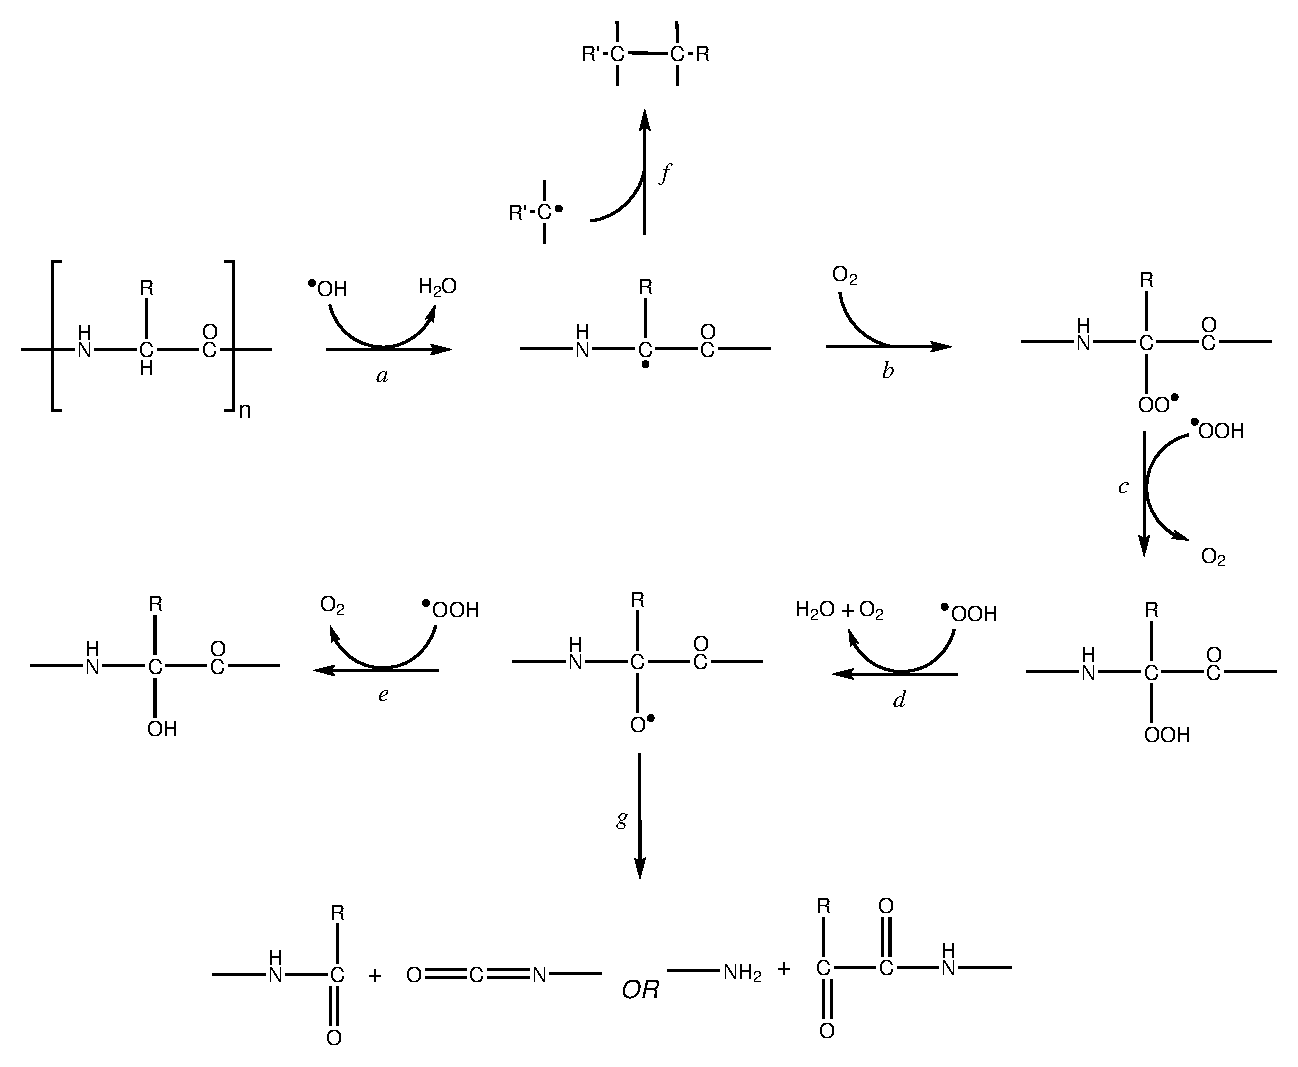
\includegraphics[width=\textwidth]{figures/proteinoxidation.eps}
  \caption[Common reactions involved in oxygen-free radical-mediated oxidation
  of proteins]{Common reaction involved in oxygen-free radical-meditated
    oxidation of proteins. The reactions are as follows: \emph{a} initiation by
    HAT by hydroxyl radical, \emph{b} radical addition of molecular oxygen,
    \emph{c} HAT with an incipient peroxyl radical, \emph{d} additional reaction
    with an incipient peroxyl radical production water and oxygen, \emph{e}
    termination by HAT with an incipient peroxyl radical, \emph{d} possible
    cross-linking mechanism of two carbon centred radicals \emph{g} possible
    fragmentation pathways of oxygen centred radical intermediate. Figure
    adapted from Reference \protect\citenum{Berlett1997}.}
  \label{fig:proteinoxidation}
  \end{center}
\end{scheme}


Nucleic acids are also susceptible to radical
damage,\cite{Halliwell2015,Valko2007} where reactions of \ch{^.OH} with the DNA
molecule having been studied in some detail. Damage can occur to both the
pyrimidine and purine bases, as well as the deoxyribose backbone. Over 20 DNA
lesions have been identified.\cite{Dizdaroglu1992,Cooke2003} The most common,
and most studied product is 8-hydroxyguanine (or the tautomer
8-oxo-2`-deoxyguanosine), which is the result of the oxidation of the guanine
nitrogenous base. This particular oxidation can results in mismatched base
pairing with adenine, contrary to the Watson-Crick model, and G$\righarrow$T and
C$\rightarrow$A substitutions can occur in the genome.\cite{Cheng1992} It is
important to realise that although there are enzymes which actively repair DNA
and remove lesions,\cite{Friedberg2005} oxidation represents the permanent
modification of genetic material which is the first step in mutagenisis,
carcinogenisis, and ageing.


Other cellular components involving polyunsaturated fatty acids are extremely
sensitive to oxidation. Specifically, the autoxidation of polyunsaturated fatty
acids and esters has been intensely
investigated.\cite{Marnett2000,Sevanian2000,Pratt2003,Spiteller2007,Ayala2014}
The radical chain reaction, illustrated in part in \ref{fig:lipidoxidation}, is
often initiated by reactions of lipids with \ch{^.OH} (Reaction $1$) forming a
pentadienyl radical. Oxygen adds rapidly (although reversibly, Reaction $2$) to
the intermediate carbon radical,\cite{Pratt2003} giving a lipid peroxyl radical
(\ch{LOO^.}). Once formed, \ch{LOO^.} can propagate to form further carbon
centred radicals (Reaction $3$), or can rearrange through a cyclisation reaction
to form an endoperoxide (Reaction $4$), reacting further to produce mainly
aldehydes, and most predominantly malondialdehyde (MDA).\cite{Valko2007} MDA is
highly reactive and has been shown to be either mutagenic or carcinogenic in
mammalian and bacterial models.\cite{Marnett2000}

\begin{scheme}
  \begin{center}
  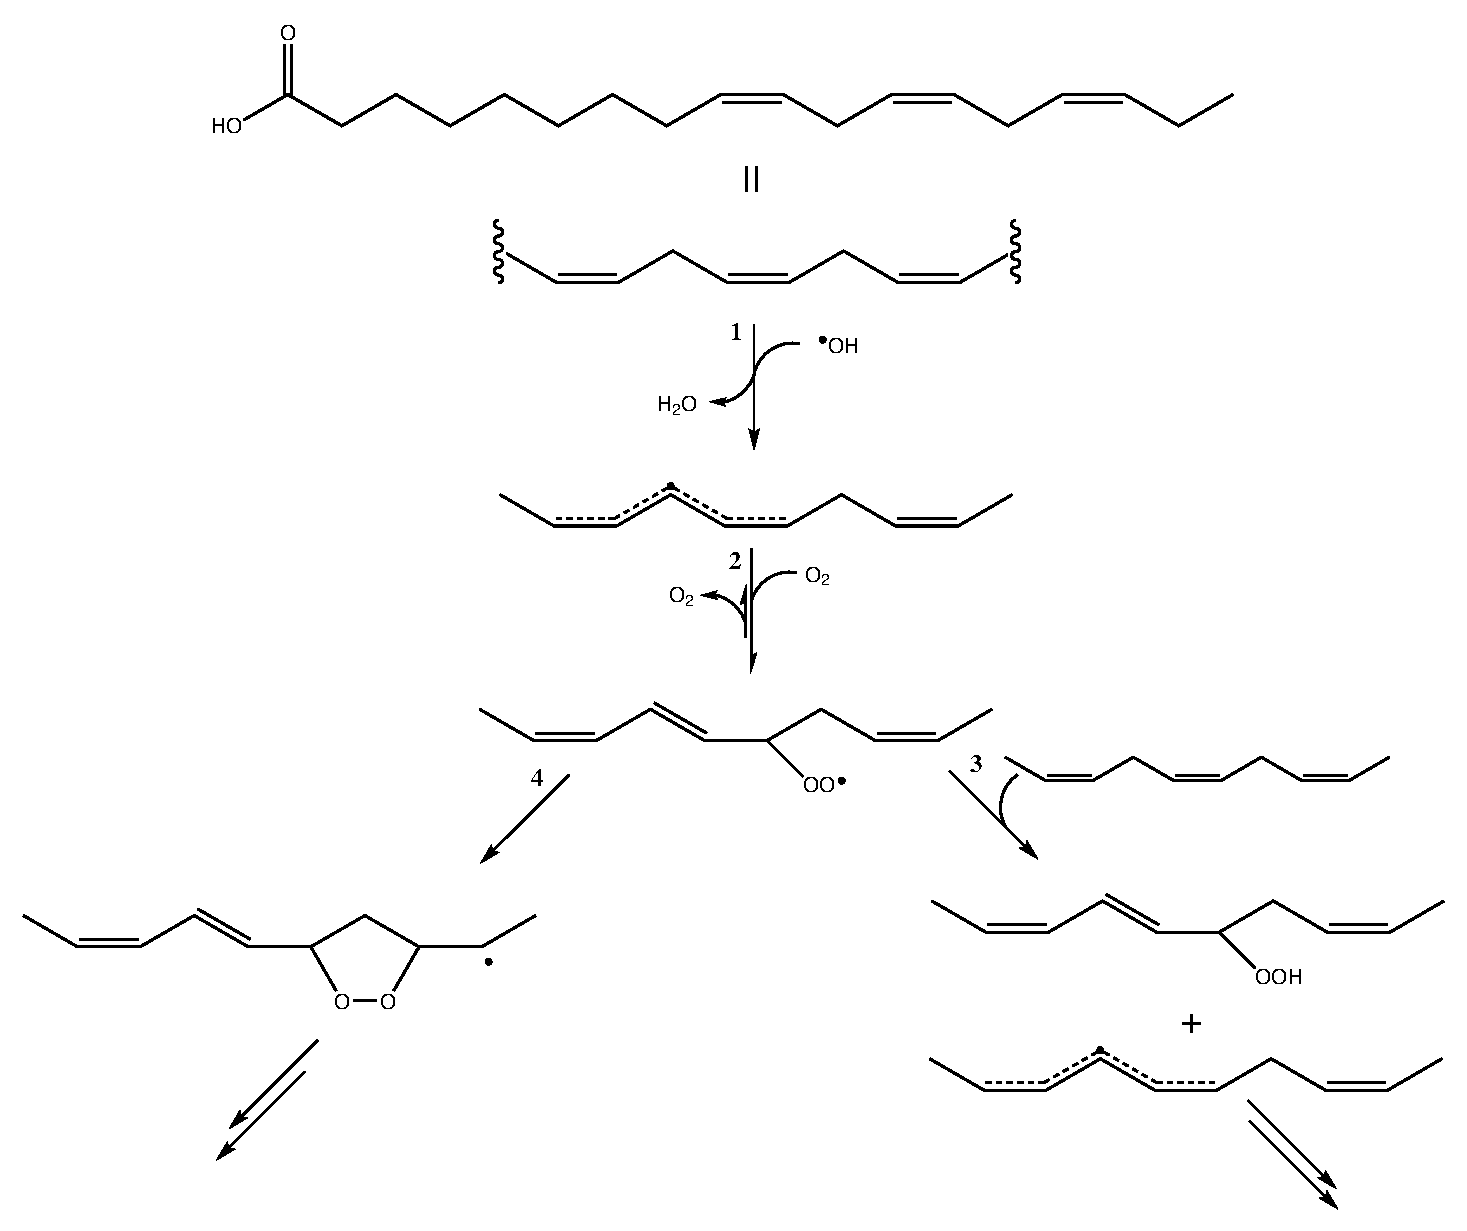
\includegraphics[width=\textwidth]{figures/lipidoxidation.eps}
  \caption[Common reactions involved in the autoxidation of fatty acids with
  linoleic acid as an example]{Common reactions involved in the autoxidation of
    fatty acids with linoleic acid as an example. The reactions are as follows:
    \textbf{1} initiation by HAT by a hydroxyl radical, \textbf{2} reversible
    addition of molecular oxygen, \texbf{3} propagation through HAT with another
    fatty acid, \textbf{4} possible cyclisation reaction leading to aldehyde
    products.}
  \label{fig:lipidoxidation}
  \end{center}
\end{scheme}


\subsection{Hydrogen atom transfer reaction in chemical processes}

Given the importance of HAT reaction in biological systems, it seems obvious for
chemists to develop means in which this tool can be used as well. Given the
highly reactive nature of free radicals, this has certainly been a challenge.
However, there exists multiple examples of utilising HAT reaction in important
energy conversion processes,\cite{Hammes-Schiffer2012} as well as in chemical
synthesis.\cite{Balcells2016,Miller2016}

Regarded as the most important scientific challenge in the modern era is the
development of alternative energy sources to fossil fuels. Given the sheer
amount of energy that the sun provides to the earth (it is estimated that every
hour the Sun provides the Earth with more energy than is consumed in a
year),\cite{Karkas2014} a tremendous amount of work has gone into developing
solar energy. Although much of what is employed today involves solar fuel cells,
work is also underway to develop an artificial photosynthetic route. That is,
rather than the plant based conversioin carbon dioxide and water into
carbohydrates, generally described by equation \ref{eq:photo},

\begin{align} 
\ch{6 CO2 + 12 H2O -> C6H12O6 + 6 O2 + 6 H2O}\label{eq:photo}
\end{align}

\noindent solar energy can be used to split water into molecular oxygen and
hydrogen \emph{via} equations \ref{eq:h2osplit1}-\ref{eq:h2osplit3}.

\begin{align} 
\ch{2 H2O &-> O2 + 4 H^+ + 4 e^-}\label{eq:h2osplit1} \\ 
\ch{4 H^+ + 4 e^- &-> 2 H2}\label{eq:h2osplit2} \\ 
\cline{1-2} 
\ch{2 H2O &-> O2 + 2 H2}\label{eq:h2osplit3}
\end{align}

The primary challenge associated with splitting \ch{H2O} by light is that the
two half-reaction are multi-electron processes. As such, an efficient process
that can do this is required. In practise this is broken into several key
problems: the process must be able to efficiently 1) absorb a photon by a
chromophore 2) form a charge separated state through a reduction catalyst, 3)
accept and accumulate two consecutive electrons to perform hydrogen reduction,
4) allow regeneration of the chromophore by an oxidation catalyst, and 5) after
four-consecutive electron transfers, the oxidation catalyst must be regenerated
by formal one-step transfer of for electrons from two water molecules to
generate one molecule of \ch{O2} and four
protons.\cite{Gust2009,Concepcion2012,Karkas2014} Many of the catalysts which
have been proposed for the oxidation and reduction steps, undergo HAT reactions
as part of their catalytic cycles, however these reactions typically take place
through a transition metal (TM) PCET mechanism, a process which is often
described as where the transfer of a proton to a ligand associated with the TM
complex, while an electron is added or removed from the metal centre. PCET in
inorganic chemistry is another fascinating area, however this thesis shall focus
on organic HAT reactions. Nonetheless, HAT/PCET remains an important process in
developing artificial photosynthetic technologies, and other alternative energy
technologies.


In organic synthesis, the replacement of specific C-H bonds (C-H bond
fictionalisation) has long been of interest. One such way to achieve this is
through radical reactions.\cite{Godula2006} Intramolecular radical reactions
were first utilised in the late 1800s when Hofmann showed that homolysis of
bromamines and chloramines lead to fictionalisation of $\delta$-methylene or
methyl groups.\jnote{citation needed, see \citet{Godula2006}} Now called the
Hofmann-L{\"o}fler-Freytag reaction, this reaction is used to form cyclic
amines, and proceeds through an intramolecular HAT, as shown in
\ref{fig:hofmann} The reaction is initiated by the cleavage of an
nitrogen-halogen bond, either by radiation or a radical initiator, followed by
an intramolecular HAT reaction that proceeds through a six-membered cyclic
transition state which can adopt an unstrained chair conformation.  Another
related reaction is the Barton reaction\cite{Barton1960} which involves
photo-initiated homolytic cleavage of an nitrite (RO-NO) bond, followed by
$\delta$-hydrogen abstraction, and radical coupling to form a $\delta$-nitroso
alcohol.

\begin{scheme}[htb]
  \begin{center}
  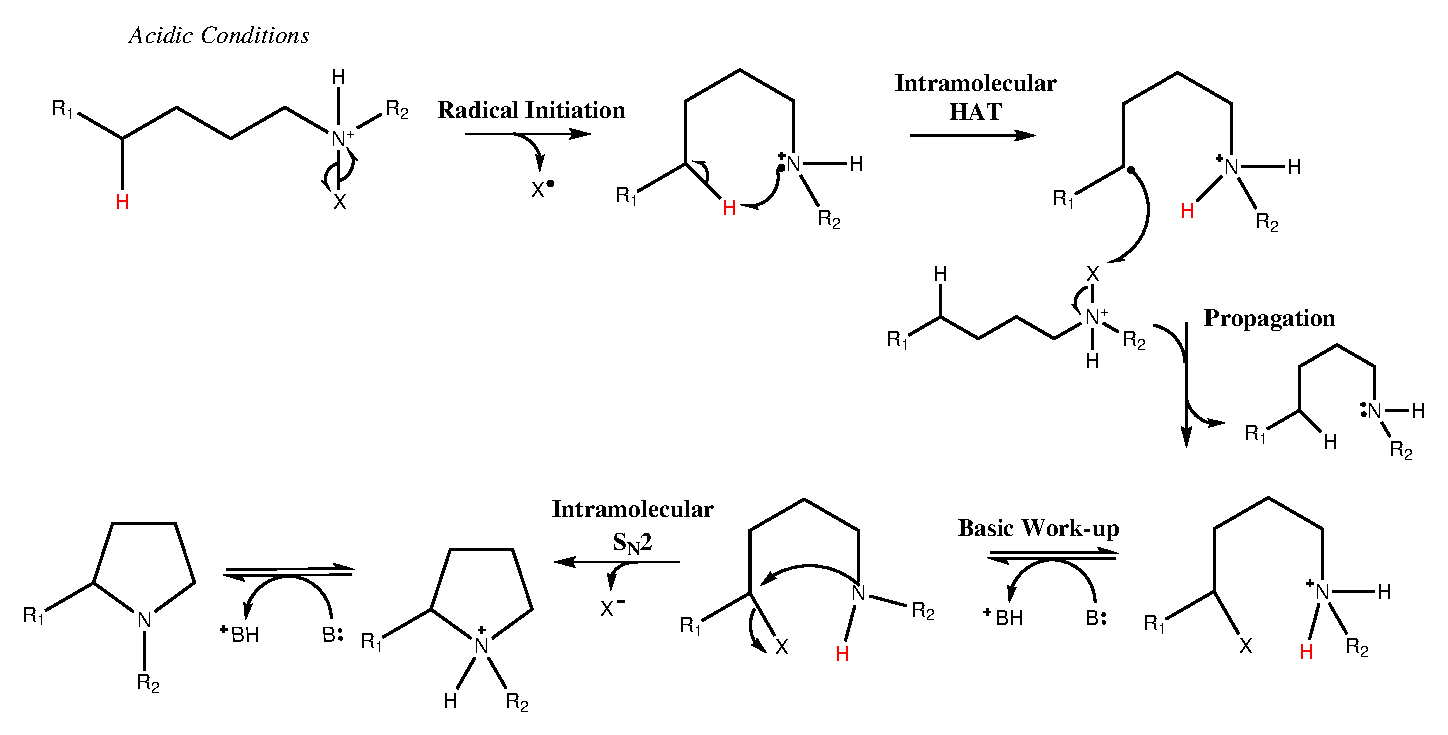
\includegraphics[width=\textwidth]{figures/hofmann.eps}
  \caption[Reaction mechanism of the Hofmann-L{\"o}fler-Freytag reaction]{
    Reaction mechanism of the Hofmann-L{\"o}fler-Freytag reaction. The reaction
    proceeds under acidic conditions so that the amine in protonated. Step one
    is radical initiation, typically through radiation or a radical initiator,
    step two is the intramolecular HAT reaction, step three is the propagation
    of the radical activating addition amines and abstracting a halide, step
    four begins the basic work up with deprotonation of the amine, followed by
    $S_N2$ attack of the $\delta$ position with a halide, and finally the second
    deprotonation of the amine centre.}
  \label{fig:hofmann}
  \end{center}
\end{scheme}

Since these early days, a great deal of work has been done, and new methods for
C-H fictionalisation have been achieved. The most commonly used technique is the
hydroxylation of C-H bonds, which then serves as a synthetic handle. This is
typically achieved through TM chemistry, which involves a highly reactive
metal-oxo intermediates responsible for triggering C-H bond cleavage, with an
inorganic PCET reaction being an essential part of the
mechanism.\cite{Groves1976} Reactions of this nature are subject to low
selectivity and complex product mixtures due to the similarly thermodynamics and
kinetics of hydroxylation and dehydrogenation pathways.\cite{Balcells2016} A
similar mechanism of metalloenzymes, which has prompted important work
investigation the selectivity and tunability of these reactions, with
considerable success. DFT studies of these reactions lead to the conclusion that
selectivity of hydroxylation/dehydrogenation could be controlled by spin
crossover.\cite{Conde2013} This once again departures from organic HAT reactions,
as are studied thesis, however this, and work by others\cite{Miller2016} is an
exemplary case where a detailed understanding of the HAT reaction mechanism can
lead to significant contributions to chemistry.

\newpage
\section{Research hypotheses and objectives}
\label{sec:hypotheses}

Hydrogen atom transfer reactions represent a simple, yet important chemical
transformation that is relevant to many fields of study. It is therefore
important that these reactions be as well defined and understood as
possible. The ideal tool for this the combined experimental and computational
study of model systems. The understanding gained from these systems should be
applicable to to other chemical species, therefore giving important insight into
the bioligical and chemical process which are studied now and in the future. The
following two chapters shall serve as the theoretical background (Chapter
\ref{ch:theory}) for the theoretical procedures employed (Chapter
\ref{ch:methods}) to investigated several key hypotheses: There exists a linear
relationship between the non-covalent binding and Arrhenius pre-factors (Chapter
\ref{ch:arrhenius}); the Bell-Evans-Polanyi Principle may be applicable for
aliphatic C-H bonds as a whole, and may (or probably doesn't now?) apply to all
other alkyl C-H bonds (Chapter \ref{ch:bdes}); and non-redox active metal cations
exhibit a chemo-protective effect against abstraction by oxygen centered
radicals in biologically and chemically relevant substrates (Chapter
\ref{ch:hat}). 

These hypotheses were explored through the following objectives:

\textbf{Chapter 4}
\begin{itemize}
\item To determine the global minimum stuctures of hydrogen-bonded pre-reaction
  complexes for near thermoneutral HAT reaction which have experimental results.

\item To determine accurate binding energies that can be used to correlate with
  experimentally determined Arrhenius pre-factors.

\item To obtain transition state structures that can be used to test or validate
  computational methods for the determination of kinetic properties of HAT
  reactions.
\end{itemize}

\textbf{Chapter 5}
\begin{itemize}
\item To obtain highly-accurate bond dissociation enthalpies for C-H bonds for
  which experimental rate constants have been determined.

\item To prepare and analyse Bell-Evans-Polanyi plots of the obtained data and
  determine if there exists two linear relationships for allylic and alkyl C-H
  bonds.
\end{itemize}

\textbf{Chapter 6}
TOMORROW
%%% Local Variables:
%%% mode: latex
%%% TeX-master: "diss"
%%% End:
